
\chapter{Experiments and Discussion}

\section{Introduction}
In this chapter, we perform different experiments for the following purposes:
\begin{itemize}
	\item to evaluate the performance of uncertainty estimation of dropout variational inference and its variants as well as Laplace approximation. Comparisons and analysis towards the results of these two kinds of approach are given.
	
	\item to evaluate performance of training a domain specific classifier, which is performing more accurately for the objects that are encountered by the robot, with different strategies for collecting training data including manual labeling and automatic labeling, where the latter one is chosen based on uncertainty estimation.
	
	\item to evaluate performance of classifier including context information via CRF.
\end{itemize}

Before looking into the results, we need to specify the details of experiments such as the dataset, evaluation metrics. Besides, the detailed parameters of the model will be reported in section of each experiment to avoid confusions.

\subsection{Dataset}
\paragraph{WRGBD\cite{lai2011large}} This dataset is a large-scale dataset of 300 household objects captured from multi-viewpoint. The objects are organized into 51 categories, some of categories and their subtrees are showed in figure \ref{fig:wrgbd1}. To note that category level recognition and detection involves classifying previously unseen objects as belonging in the same category as objects that have previously been seen(e.g., coffee
mug). Instance level recognition and detection is identifying
whether an object is physically the same object that has
previously been seen. Therefore the overlapping of features in category classification is larger than that in instance classification. The setup of dataset is, that each object was placed on a turn table and captured from a systematically sampled view hemisphere with $15^{\circ}$ step in elevation (from $30^{\circ}$to $60^{\circ}$) and $2^\circ$ step in azimuth (from $0^\circ$ to $360^\circ$) (cf. figure \ref{fig:wrgbd2}).
\begin{figure}[h!]
	\begin{center}
		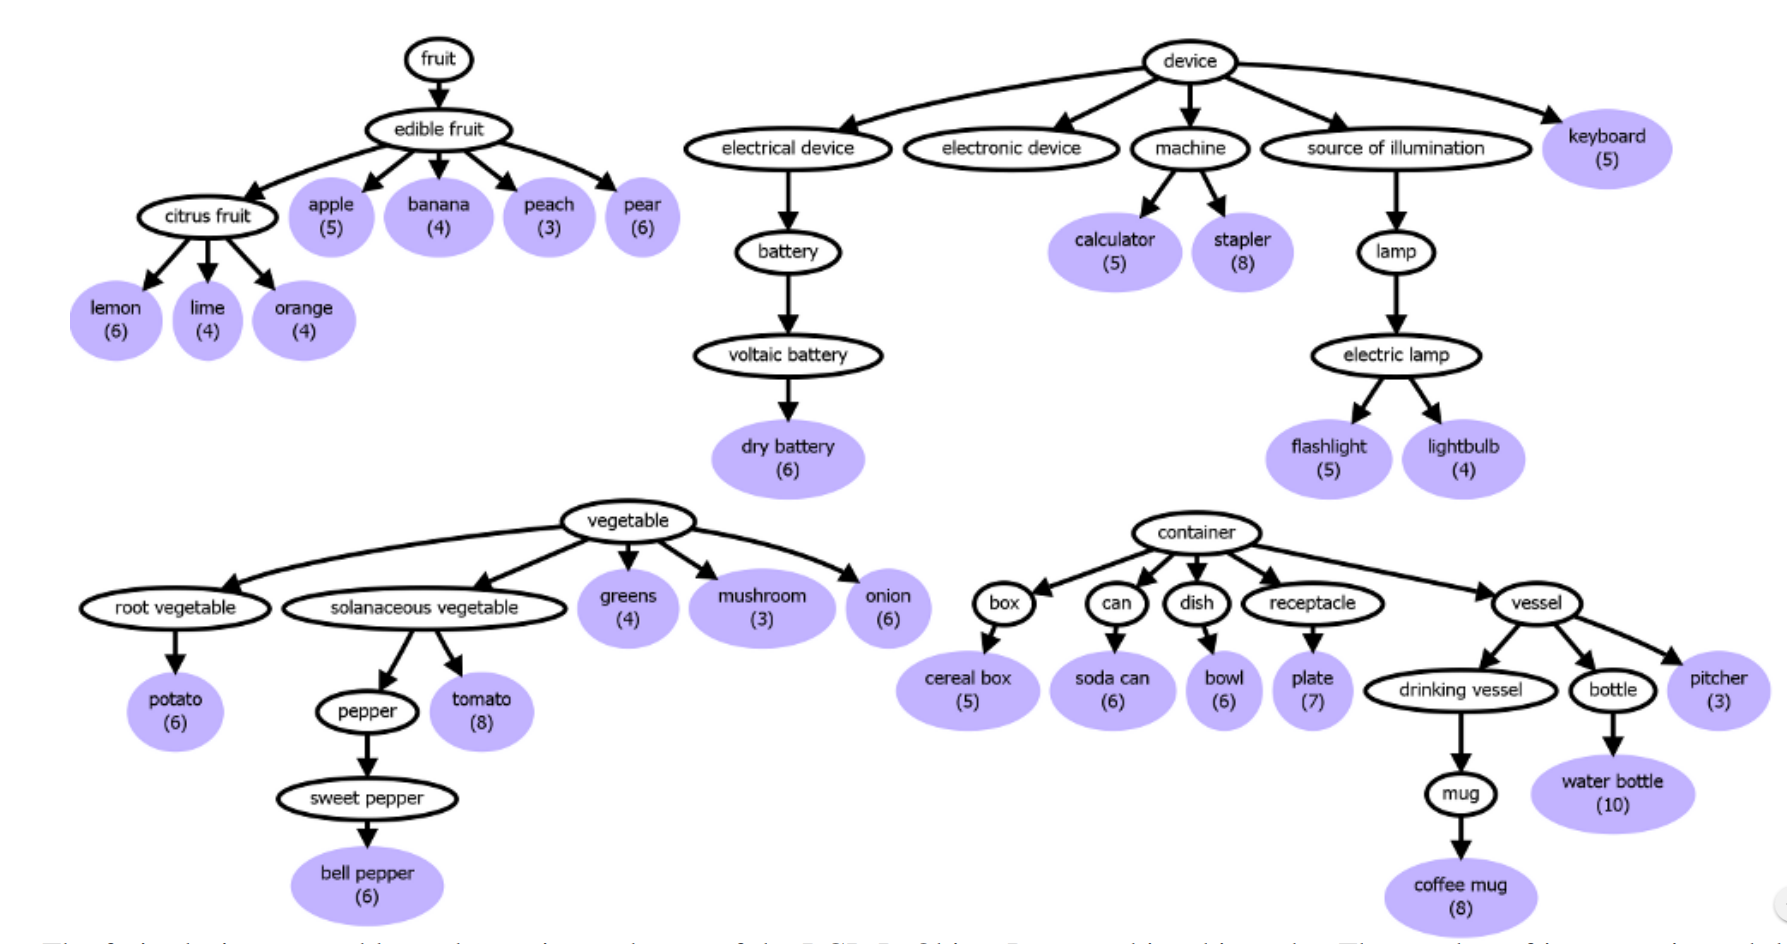
\includegraphics[height=7cm, width=14cm]{wrgbd1}
		\caption{The fruit, device, vegetable, and container subtrees of the RGB-D Object Dataset object hierarchy, the shaded ellipse represent categories and number inside parenthesis denotes the number of instances within this category\cite{lai2011large}.}		
		\label{fig:wrgbd1}
	\end{center}
\end{figure}
 \begin{figure}[h!]
 	\begin{center}
 		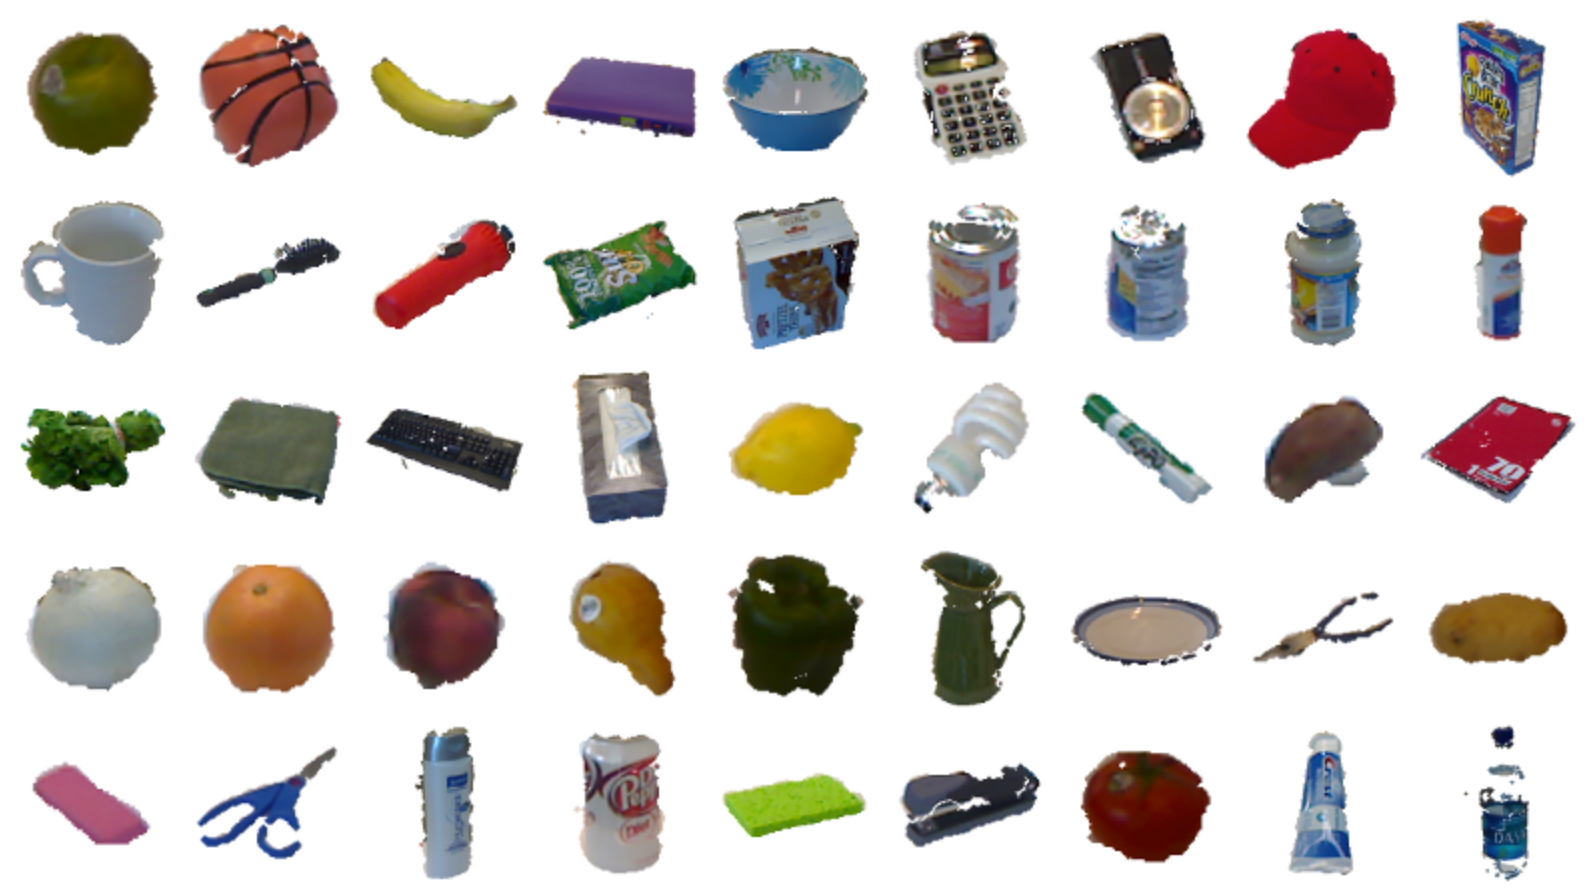
\includegraphics[height=6.5cm, width=12cm]{wrgbd2}
 		\caption{Example of masked images from subset of objects in WRGBD dataset.}		
 		\label{fig:wrgbd2}
 	\end{center}
 \end{figure}
 


\paragraph{UniHB} To simulate application-specific situation in robotic deployment, we recorded a similar dataset by putting objects on a turn table in front of the robot and recording partial views of objects this way. We follow the same methodology as \cite{lai2011large} suggests for WRGBD, but with only one object instance for each category in the dataset. This analogue of WRGBD dataset is called the IAI-ODU dataset of UniHB. While the UniHB dataset's setup strives to mimic the WRGBD one, the differing capturing conditions such as different equipment and light conditions even appearances of objects, result in a slightly modified feature space, thus yielding a significant drop on classification accuracy. \textbf{[TODO:} add examples of objects in WRGBD and UniHB.] In addition to the existing 51 categories, there are 28 novel objects that do not belong to the 51 categories and these objects are treated as out-of-distribution(OOD) data for testing uncertainty estimation of the model. To note that these novel objects are recorded in a slight different way, that is, their view points are sampled with $15^{\circ}$ step in elevation (from $30^{\circ}$to $60^{\circ}$) and $5^\circ$ step in azimuth (from $0^\circ$ to $360^\circ$)

\paragraph{T-LESS\cite{hodan2017tless}}


\subsection{Uncertainty measures}
For each prediction, we can obtain one predictive probability distribution from our model with equation \ref{marginalization_test}. In order to quantify uncertainty of the prediction,there are different metrics to measure the uncertainty of prediction, which are introduced in the following. We define $x^\star$ as one test data sample and $\mathcal D$ as our training set. 
\paragraph{Confidence} is defined as the maximum probability of the output predictive distribution, whose index is the class prediction.

\begin{equation}\label{confidence}	
\begin{aligned}
conf = \max_c \big[ p(y=c|x^\star, \mathcal D) \big]
\end{aligned}
\end{equation}
where $conf \in [0,1]$, $c \in \mathcal P = \{0,...,|\mathcal P|-1\}$, and $\mathcal P$ represents output space in which label is expressed as number index which is transformed into one-hot representation in computation of objective function. The larger this quantity is, the less uncertainty the prediction is. 

\paragraph{Predictive entropy} is quantity that captures the average amount information contained in predictive distribution: 
\begin{equation}\label{entropy}	
\begin{aligned}
\mathcal H[p(y|x^\star, \mathcal D)] = -\sum_{c}p(y=c|x^\star, \mathcal D)\text{log}p(y=c|x^\star, \mathcal D)
\end{aligned}
\end{equation}
where $c$ is the possible class $y$ can take, $\mathcal H(\cdot) \in [0, \text{log}{|\mathcal P|}]$, the larger this quantity is, the more uncertainty the prediction is.

\paragraph{Mutual information}
Mutual information between the prediction $y$ and the weights posterior offers a different uncertainty measure. This measure is widely used in active learning tasks\cite{houlsby2011bayesian}.
\begin{equation}\label{mi}	
\begin{aligned}
\mathcal I[y,\bld \omega|x^\star, \mathcal D] &= \mathcal H[y|x^\star, \mathcal D] - \mathbb E_{p(\bld \omega| \mathcal D)}\big[\mathcal H[y|x^\star, \bld \omega] \big] \\
&= -\sum_{c}p(y=c|x^\star, \mathcal D)\text{log}p(y=c|x^\star, \mathcal D) \\ &+ \mathbb E_{p(\bld \omega|\mathcal D)}[-\sum_{c}p(y=c|x^\star, \bld \omega)\text{log}p(y=c|x^\star, \bld \omega)] \\
&\approx -\sum_{c}p(y=c|x^\star, \mathcal D)\text{log}p(y=c|x^\star, \mathcal D) \\ &+ \mathbb E_{q(\bld \omega)}[-\sum_{c}p(y=c|x^\star, \bld \omega)\text{log}p(y=c|x^\star, \bld \omega)]
\end{aligned}
\end{equation}
where $\mathcal I(\cdot) \in [0,\text{log}{|\mathcal P|}]$.
This quantity consider the effect of approximate posterior distribution directly. Compared with aforementioned uncertainty measures, this one should be able to capture the model uncertainty more accurately. To think about it intuitively, this quantity measure the information gain between the entropy of predictive output distribution and the expected entropy of output distribution w.r.t. weights posterior. It will be low only if the predictive distribution agrees with most of possible models(weights realizations), which means that the model is sure about its prediction. Otherwise, it will be high because most of possible models do not agree with each other and thus the predictive distribution will be more uniform.

\subsection{Evaluation metrics}
As is stated in \cite{gneiting2007probabilistic}, the goal of probabilistic prediction is to maximize the sharpness of predictive prediction subject to calibration. Calibration refers to the statistical consistency between the predictive probability and the occurrence of observations. Therefore we employ different metrics including both the accuracy and other quantities related to calibration as well as summary of accuracy and calibration. Additionally, we also employ histogram and diagram to express the results visually. While the visual one can show us the results more directly, the quantitive one can enable us to evaluate the results more objective. The comparison between them can also help us to examine if visual metrics are corresponding to the numerical metrics and thus provide more insights in evaluating uncertainty estimation. 

\paragraph{Uncertainty histogram} is a intuitive visual representation for analyzing the statistics of the uncertainty estimation. Compared with normal histogram, there is one difference to stress. In order to make visual effect more intuitive, for each type of predictions, the \textbf{normalizer} the total number of this type of predictions instead of the entire dataset. More concretely, we have three types of predictions when plotting the histogram, which are correct predictions, miss-classifications and out-of-distribution. The range of y axis is $[0,1]$  and range of x axis is range of specific uncertainty.

\paragraph{Reliability diagram and expectation calibration error} is a visual representation of model \textbf{calibration}\cite{guo2017calibration}, which plot the frequency of success(accuracy of predictions in specific bin) as a function of confidence. If the model is perfectly calibrated, this function should be overlapping with the diagonal line. 
In order to have this plot, we firstly group the predictions into M interval bins w.r.t. confidence. We use M=20 in this work. Then calculate the accuracy of predictions in each bin.

Furthermore, in order to obtain a more objective measure of calibration quality, we can compute the expected calibration error by computing the weighted average of difference between accuracy and confidence:
\begin{equation}
ECE = \sum_{m=1}^{M}\frac{|B_m|}{n}|acc(B_m) - conf(B_m)|
\end{equation}
where $n$ is the number of samples, and $acc(B_m)$ represents the accuracy of samples, $conf(B_m)$ the average predicted confidence of samples in $m$-th bin. We can see that this metric measures the inconsistency between the statistics and predictive distribution. To note that this metric only considers the calibration quality instead of accuracy. 


\paragraph{Proper scoring rules} 
Scoring rules provides a \textbf{summary} measures for the evaluation of probabilistic forecasts by assigning a numerical score based on the predictive distribution and real distribution of event we want to predict. Because we want to make predictions for the future and also have a suitable measures of the uncertainty associated with them(  see \cite{gneiting2007strictly} for a review). Let's define the scoring rule as a function $\mathcal S(p(y|\bld x), (y|\bld x))$ that evaluates the quality of predictive distribution $p(y|\bld x)$ relative to an event $y|\bld x \sim q(y|\bld x)$ where $q(y|\bld x)$ represents the true distribution over $(y|\bld x)$. Consequently, the expected scoring rule is:
\begin{equation}\label{scoring rule}
	\mathcal S(p, q) = \int q(y| \bld x) \mathcal S(p,(y|\bld x))dy
\end{equation}
$\mathcal S(p,q)$ is proper if $\mathcal S(p,q) \leq S(q,q)$, with equality held if and only if $p(y|\bld x) = q(y|\bld x)$. Here we adopt two simple and famous proper scoring rules:
\begin{itemize}
	\item test NLL(test negative log likelihood):NLL is a popular metric for evaluating predictive uncertainty	\cite{quinonero2005evaluating}. This metric considers aforementioned confidence as likelihood. The smaller this metric is, the better the predictive distribution is.
	\begin{equation} \label{nll}
		NLL = -\frac{1}{|\mathcal D_{test}|}\sum_{i=1}^{|\mathcal D_{test}|}\text{log}(p(y_i = c_i|\bld x_i))
	\end{equation}
	where $c_i$ is the ground truth label for $\bld x_i$.	
	\item Brier score is the mean squared error between the target distribution(one-hot encoding label) and predictive distribution:
	\begin{equation} \label{bs}
	BS = -\frac{1}{|\mathcal D_{test}|}\sum_{i=1}^{|\mathcal D_{test}|}(\bld y^{gt}_i - p(\bld y_i|\bld x_i))^2
	\end{equation}
	where $\bld y^{gt}_i$ is the one-hot encoding ground truth label for $\bld x_i$. 
	
\end{itemize}

\paragraph{Area under Receiver Operating Curve(AUROC)} Since one of our goals is to choose automatically labeled data based on uncertainty estimation, it's better to evaluate the discriminability between correct predictions and false predictions as well as out-of distribution samples. Therefore we consider another two metrics for this purpose, that are AUROC and AUPR.

ROC describes the relationship between true positive rate($tpr=\frac{tp}{tp+fn}$) and false positive rate($fpr=\frac{fp}{fp+tn}$). Moreover, AUROC can be interpreted as the probability that a positive samples has a greater score than a negative samples.

\paragraph{Area under Precision Recall Curve(AUPR)} Because the normalizers of two rates in ROC have nothing to do with each other, when these two normalizers differs too much. AUROC can provide misleading conclusion. For example, if the number of negative predictions is much higher than positive one, the AUROC could still be high, but in fact there are still many false positives. Therefore another evaluation metric is employed, that is AUPR. AUPR describes the relationship between precision($pr = \frac{tp}{tp+fp}$) and recall($tpr=\frac{tp}{tp+fn}$), which adjusts for these different base numbers. To note that, we treat the correct predictions as positive samples.

\section{Uncertainty estimation experiments}
\subsection{Experiments \RNum{1}}
In this experiments, we want to evaluate our model on a relatively easy task at first, which means that the appearances of different categories as well as the out-of-distribution categories are highly discriminable. Therefore we separate WRGBD dataset into two subsets based on the instance label. Subset \RNum{1} contains objects with instance label from 0 to 199 (assuming that here we use index to denote the instance label) and Subset \RNum{2} contains objects with instance label from 200 to 299. 

We train our model with objects captured in elevation $30^\circ$ and $60^\circ$ of Subset \RNum{1} (in which we split off 20\% of training set as validation set for model selection in training) and test the model on objects captured in elevation $45^\circ$ of both Subset \RNum{1} and Subset \RNum{2}. In this experiment, the objects in Subset \RNum{2} serve as out-of-distribution samples because they are not present in training.

In the following we can see different evaluation metrics in this experiment from original ResNet50, dropout variational inference and Laplace approximation, respectively.


\subsection{Experiments \RNum{2}}
In this experiment, we evaluate our model on a more difficult task. The difficulties are expressed in two aspects, firstly, the task is category recognition instead of instance recognition in Experiment \RNum{1}, which means that the model is confronted with classes with more overlaps and thus more abstract concept needed to learn. Second, since we want to simulate robotic deployment situation, the UniHB dataset with slight domain gap to WRGBD is employed to achieve this goal. This means that the uncertainty estimation should not only be able to perform well on dataset with same distribution, but also to generalize well to dataset with domain gap although the accuracy may drop a lot in this situation.

Accordingly, we use the entire WRBD dataset including all view points to train our model (in which we split off 20\% of training set as validation set for model selection in training). Regarding UniHB dataset, we treat objects captured in elevation $30^\circ$ and $60^\circ$ as adaptation set and test performance of uncertainty estimation on this set. The $45^\circ$ objects are used for final testing after we fine-tune the model with subset of adaptation set to obtain a domain specific model which is experiment in next section.

\subsection{Experiments \RNum{3}}


\subsection{Ablation study}

\section{Automatic labeling experiments}
\subsection{Experiments settings}
\subsection{Results}
\subsection{Analysis}


\section{Context-based improvement experiments}
\subsection{Experiments settings}
\subsection{Results}
\subsection{Analysis}